%%% Local Variables:
%%% mode: latex
%%% TeX-master: "../main"
%%% coding: utf-8
%%% End:
% !TEX TS-program = pdflatexmk
% !TEX encoding = UTF-8 Unicode
% !TEX root = ../main.tex

The main goal is to implement a web-based path tracer addressing the problem of the large number of variants for CAD-based product visualization leveraging data close to the production CAD models.

The result of this work consists of multiple parts. The report serves as the primary documentation of the work, but does not contain the different details. The library and detailed code documentation are published under the MIT license on GitHub. See \url{https://www.github.com/StuckiSimon/strahl}. In addition, a dedicated short-paper has been published for WEB3D '24: The 29th International ACM Conference on 3D Web Technology \cite{ownShortPaper}. The short-paper includes the main insights and results of this work.

This section contains references to the implementation of the path tracer. References are formatted in a consistent manner and can be searched for in the code. All relevant places are marked in code using the same reference. For example \coderef{ABC} refers to the code with the same comment.

\section{Scene Description}
Lights, Materials, Camera, Objects
\section{Implementation}

The goal of the implementation is to be compatible with a large variety of devices and make the setup for consumers simple. Therefore, it is implemented and tested mainly in Chrome, which uses \gls{Dawn} as the underlying implementation of WebGPU. Most notably, this means that dedicated features from other implementations such as \gls{wgpu} cannot be used. Neither can experimental extensions be leveraged.

\subsection{Ray Tracing}

\subsubsection{OpenPBR}

The \gls{OpenPBR} standard is based on an \gls{uber shader} approach. This differs from node-based approaches such as \gls{MaterialX} in that it uses a fixed set of inputs which can be configured. This approach offers a good balance between flexibility and performance.

The surface shading method is based on \gls{OpenPBR} reference implementation in \gls{MaterialX} as well as the reference viewer by Portsmouth \cite{openPbrViewer}.

\subsubsection{RGB, Spectral}
\subsubsection{Memory Management}

In order to address memory alignment, as described in \autoref{ch:memoryAlignmentTheory}, the path tracer uses \texttt{webgpu-utils} \cite{webgpuUtilsLib}. The library enables a straightforward way to map data to buffers and align them correctly. See \coderef{MEMORY-VIEW} for creation of definition and \coderef{BUFFER-MAPPING} for mapping of data to buffers.

\todo{Memory Management (GPU+CPU)}

\subsection{View Projection}

For many applications, especially photorealistic rendering, perspective projection is used. Based on the assessed use cases, the path tracer uses perspective projection only. See \coderef{VIEWPROJECTION} for implementation.

\subsection{Random Number Generator}

The path tracer uses PCG-RXS-M-XS variant as described by O’Neill \cite{o2014pcg} in combination with Xorshift as described by Marsaglia \cite{marsaglia2003xorshift}. See \coderef{RNG} for implementation.

In order to set up the Monte Carlo method, the \gls{RNG} needs to be employed in a suitable manner. As it is a pseudorandom generator, it necessitates a seed to start the generation. If the seed is identical for all pixels, the results of a single sample will frequently share similar patterns in adjacent surfaces as shown in \autoref{fig:rngBadSeed}. The result for independent seeds differs in a stark manner as shown in \autoref{fig:rngGoodSeed}.

\begin{figure}[H]
    \centering
    \begin{subfigure}[b]{0.45\textwidth}
        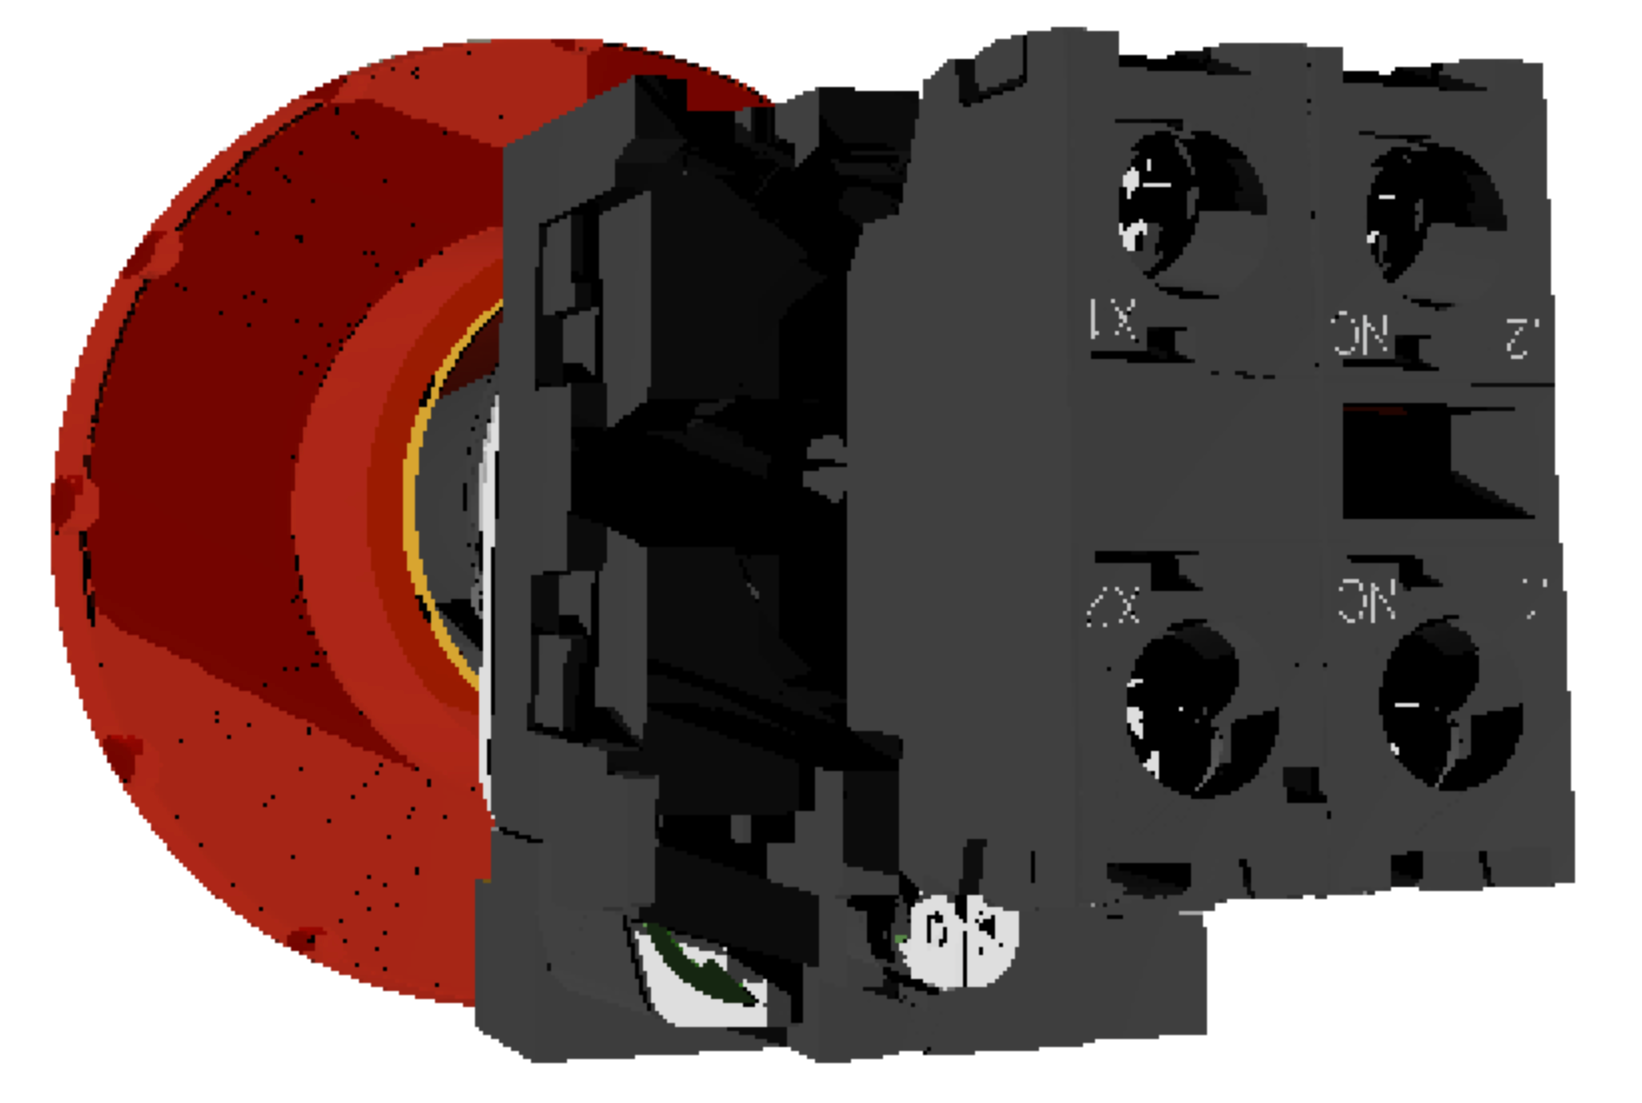
\includegraphics[width=\textwidth]{resources/single-sample-bad-seed.png}
        \caption{identical seed for all pixels}
        \label{fig:rngBadSeed}
    \end{subfigure}
    \hfill
    \begin{subfigure}[b]{0.45\textwidth}
        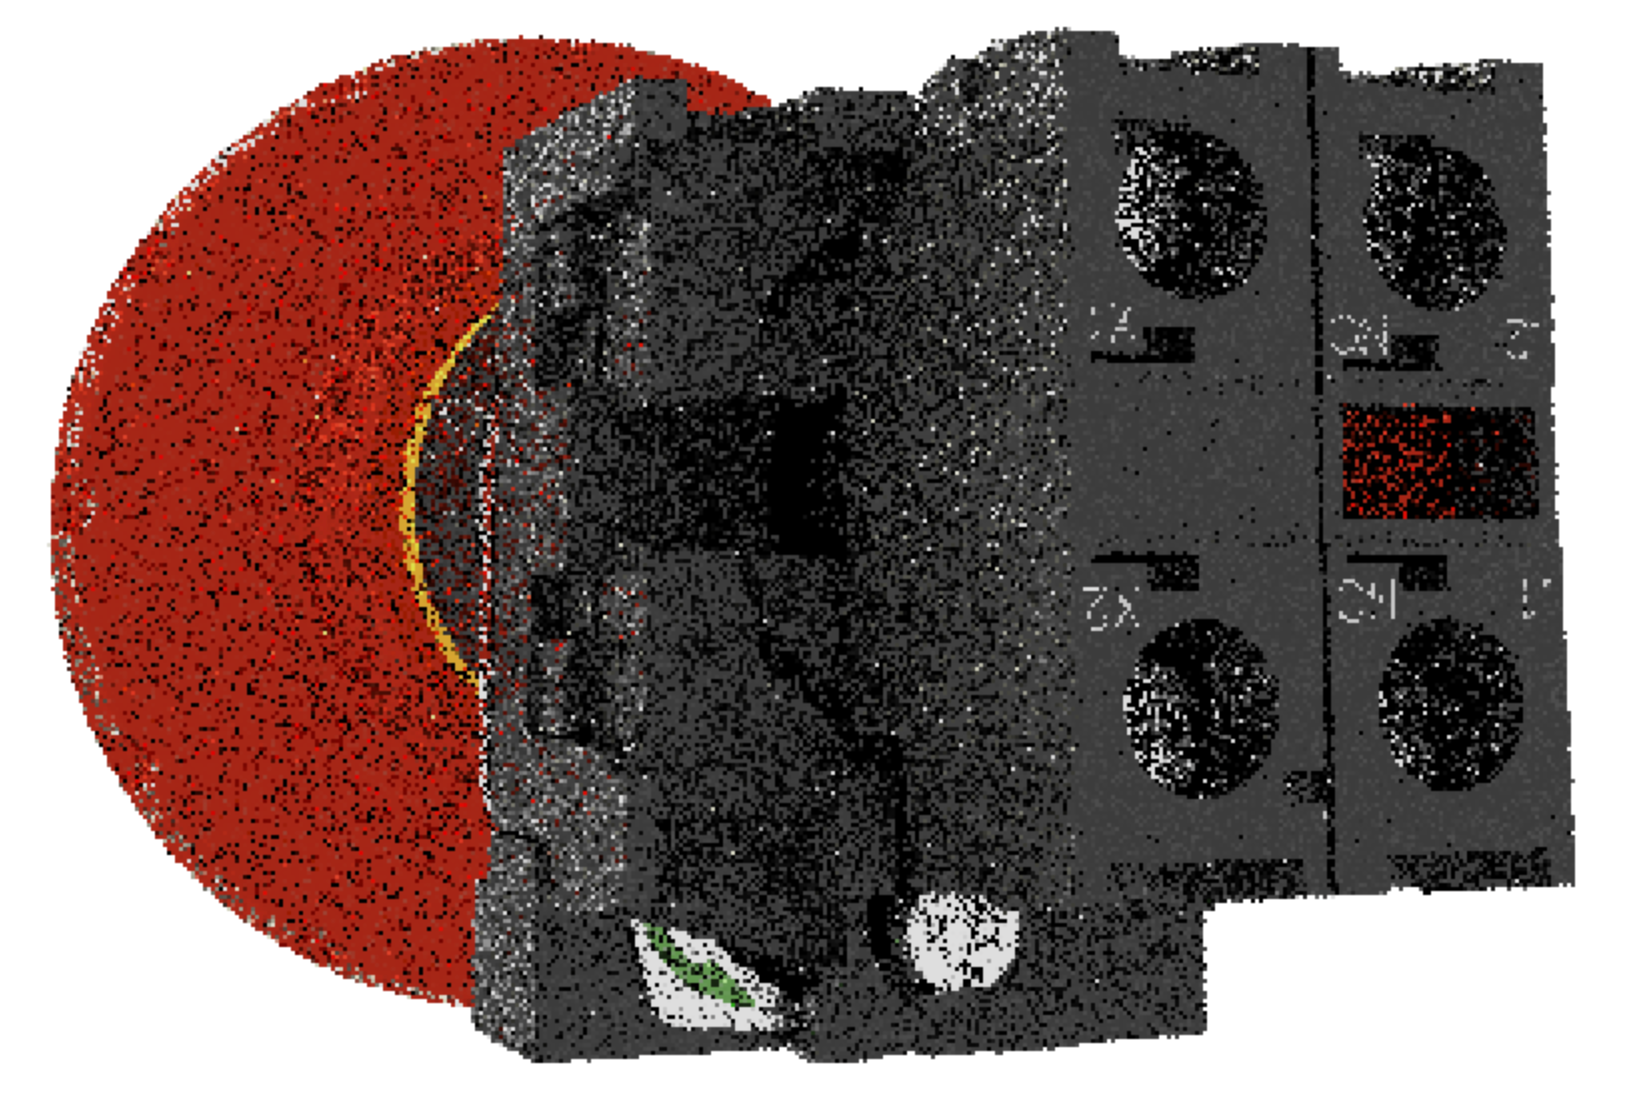
\includegraphics[width=\textwidth]{resources/single-sample-good-seed.png}
        \caption{independent seed for every pixel}
        \label{fig:rngGoodSeed}
    \end{subfigure}
    \caption{Both images consist of only one sample.}
    \label{fig:rngSeed}
\end{figure}

When increasing the sample count, the differences in the setup remain visible. Adjacent surfaces show similar patterns as shown in \autoref{fig:rngNoiseArtifactsHighlightsBadNoisy}, which resemble image compression artifacts encountered in aggressively compressed \fGlspl{JPEG}{\e{Joint Photographic Experts Group}, common method for lossy image compression}. In contrast, the renderings with independent seeds show stark differences in adjacent pixels akin to noise as shown in \autoref{fig:rngNoiseArtifactsHighlightsGoodNoisy}. As shown in \autoref{fig:rngNoiseArtifactsHighlightsBadAnti} compared to \autoref{fig:rngNoiseArtifactsHighlightsGoodAnti}, the anti-aliasing is less noticeable when using independent seeds.

\begin{figure}[H]
    \centering
    \hspace*{2cm}
    \begin{subfigure}[t]{0.3\textwidth}
        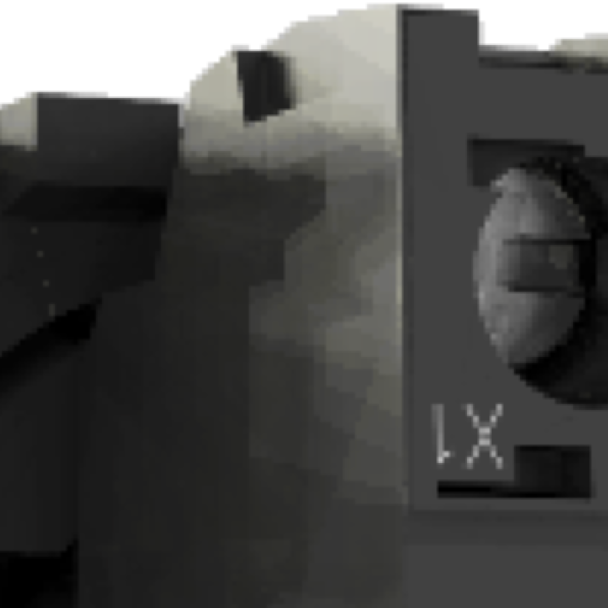
\includegraphics[width=\textwidth]{resources/bad-seed-noisy.png}
        \caption{Renderings which resemble lossy image compression artifacts.}
        \label{fig:rngNoiseArtifactsHighlightsBadNoisy}
    \end{subfigure}
    \hfill
    \begin{subfigure}[t]{0.3\textwidth}
        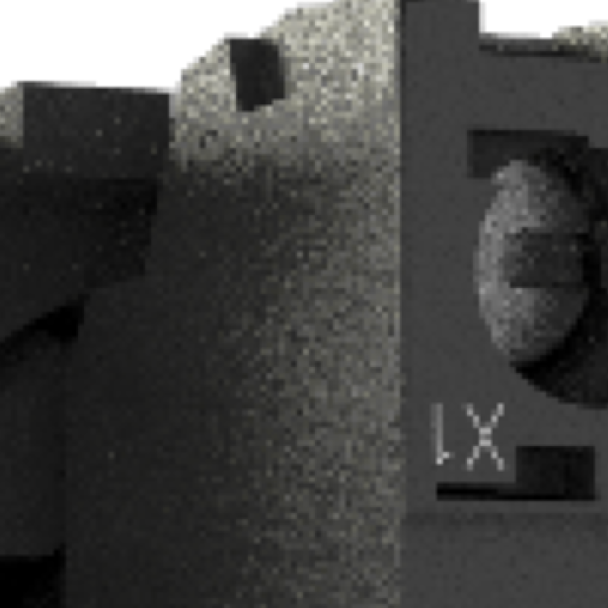
\includegraphics[width=\textwidth]{resources/good-seed-noisy.png}
        \caption{Noisy renderings with stark differences in adjacent pixels.}
        \label{fig:rngNoiseArtifactsHighlightsGoodNoisy}
    \end{subfigure}
    \hspace*{2cm}
    \vfill
    \vspace*{0.5cm}
    \hspace*{2cm}
    \begin{subfigure}[t]{0.3\textwidth}
        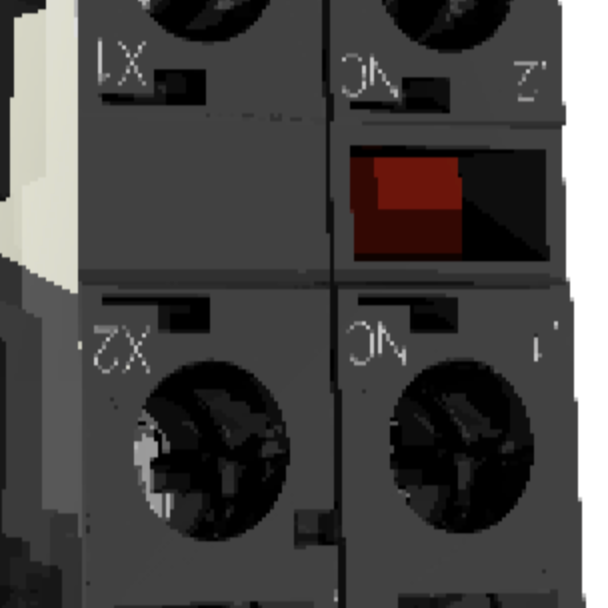
\includegraphics[width=\textwidth]{resources/bad-seed-anti-aliasing.png}
        \caption{On the right side, anti-aliasing is rather noticeable.}
        \label{fig:rngNoiseArtifactsHighlightsBadAnti}
    \end{subfigure}
    \hfill
    \begin{subfigure}[t]{0.3\textwidth}
        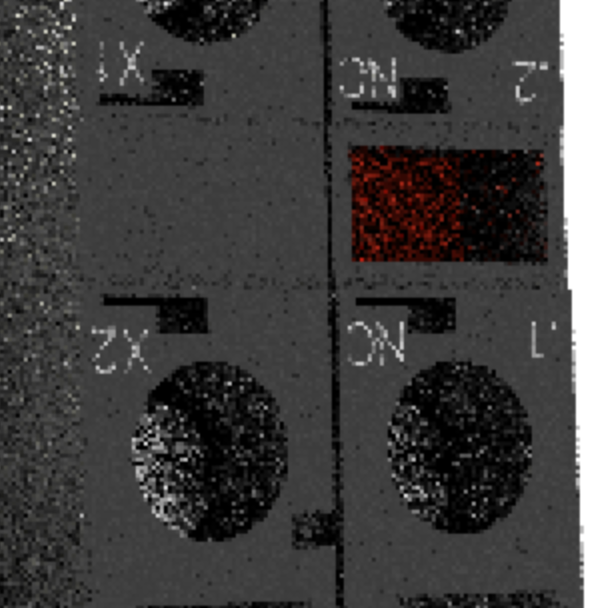
\includegraphics[width=\textwidth]{resources/good-seed-anti-aliasing.png}
        \caption{On the right side, anti-aliasing is less noticeable.}
        \label{fig:rngNoiseArtifactsHighlightsGoodAnti}
    \end{subfigure}
    \hspace*{2cm}
    \caption{Magnified images of renderings with low sample count showing difference based on seed setup. Left column has identical seed for all pixels of a sample, but varying seeds for different samples. Right column has independent seeds for every pixel of a sample as well as across samples.}
    \label{fig:rngNoiseArtifactsHighlights}
\end{figure}

\subsection{Intersection Testing}

For \gls{BVH} construction, well-established solutions for the web are available. The path tracer uses \texttt{three-mesh-bvh} \cite{threeMeshBvh}. This method builds the \gls{BVH} on the \gls{CPU}, the code for transfering the \gls{BVH} to the \gls{GPU} is in \coderef{BVH-TRANSFER}, intersection tests are implemented in \gls{WGSL}, see \coderef{BVH-TESTS}.

\subsection{Anti-Aliasing}

The implementation of the strategy indicated in \ref{sec:anti-aliasing} is implemented in \coderef{ALIASING}.


\subsection{WebGPU}
\subsection{Integration}
\section{Use Case Scenarios}
\section{Performance}